\chapter{Implementation}
This chapter describes how the design was implemented in the prototype. Furthermore, it describes how the narration system, dubbed the narration-o-matic, was created.

\section{Virtual Reality with Oculus}
    Getting started with Oculus in the Unity game engine is fairly straightforward, simply putting their SDK into unity, with a package made for the engine, allows one to put in a VR camera and an avatar, containing the hands and body of the user.
    \subsection{Burger Eating}
        For grabbing the burger, Oculus has created two useful scripts, \mintinline{csharp}{OVRGrabbable}, and \mintinline{csharp}{OVRGrabber}. \mintinline{csharp}{OVRGrabbable} is put onto the burger, and \mintinline{csharp}{OVRGrabber} then activates the script when the trigger button on the Oculus touch controller is pressed if the hand is inside the burger. The burger object is then re-parented to the hand that activated it, allowing it to be moved with the hand. Then, having a trigger collider in the face of the VR camera rig, activating the eating behaviour in the narration-o-matic, when the burger is entering it.


\section{Narration-o-matic}
    For handling the narration mentioned in the design, a robust system was needed, something that could handle many different clips, and allowing for pacing out the clips and pauses between the different narration pieces. It should also allow for easier changing between the two version, for an an easier conductable test.
    
    The resulting system, is the narration-o-matic, and drag and drop solution, allowing for quick setup, and easy changes. The system allows for actions being executed when a sound clip starts playing, like spawning birds, or starting a tornado. A general overview of the structure of the narration-o-matic can be seen in \autoref{fig:narration-o-matic}, showing that each of the five narration pieces, contains 3 Intermixed clips and 3 Overloaded clips, with the first piece also containing an introduction clip, that introduces the radio host and program.
    
    \begin{figure}[H]
        \centering
        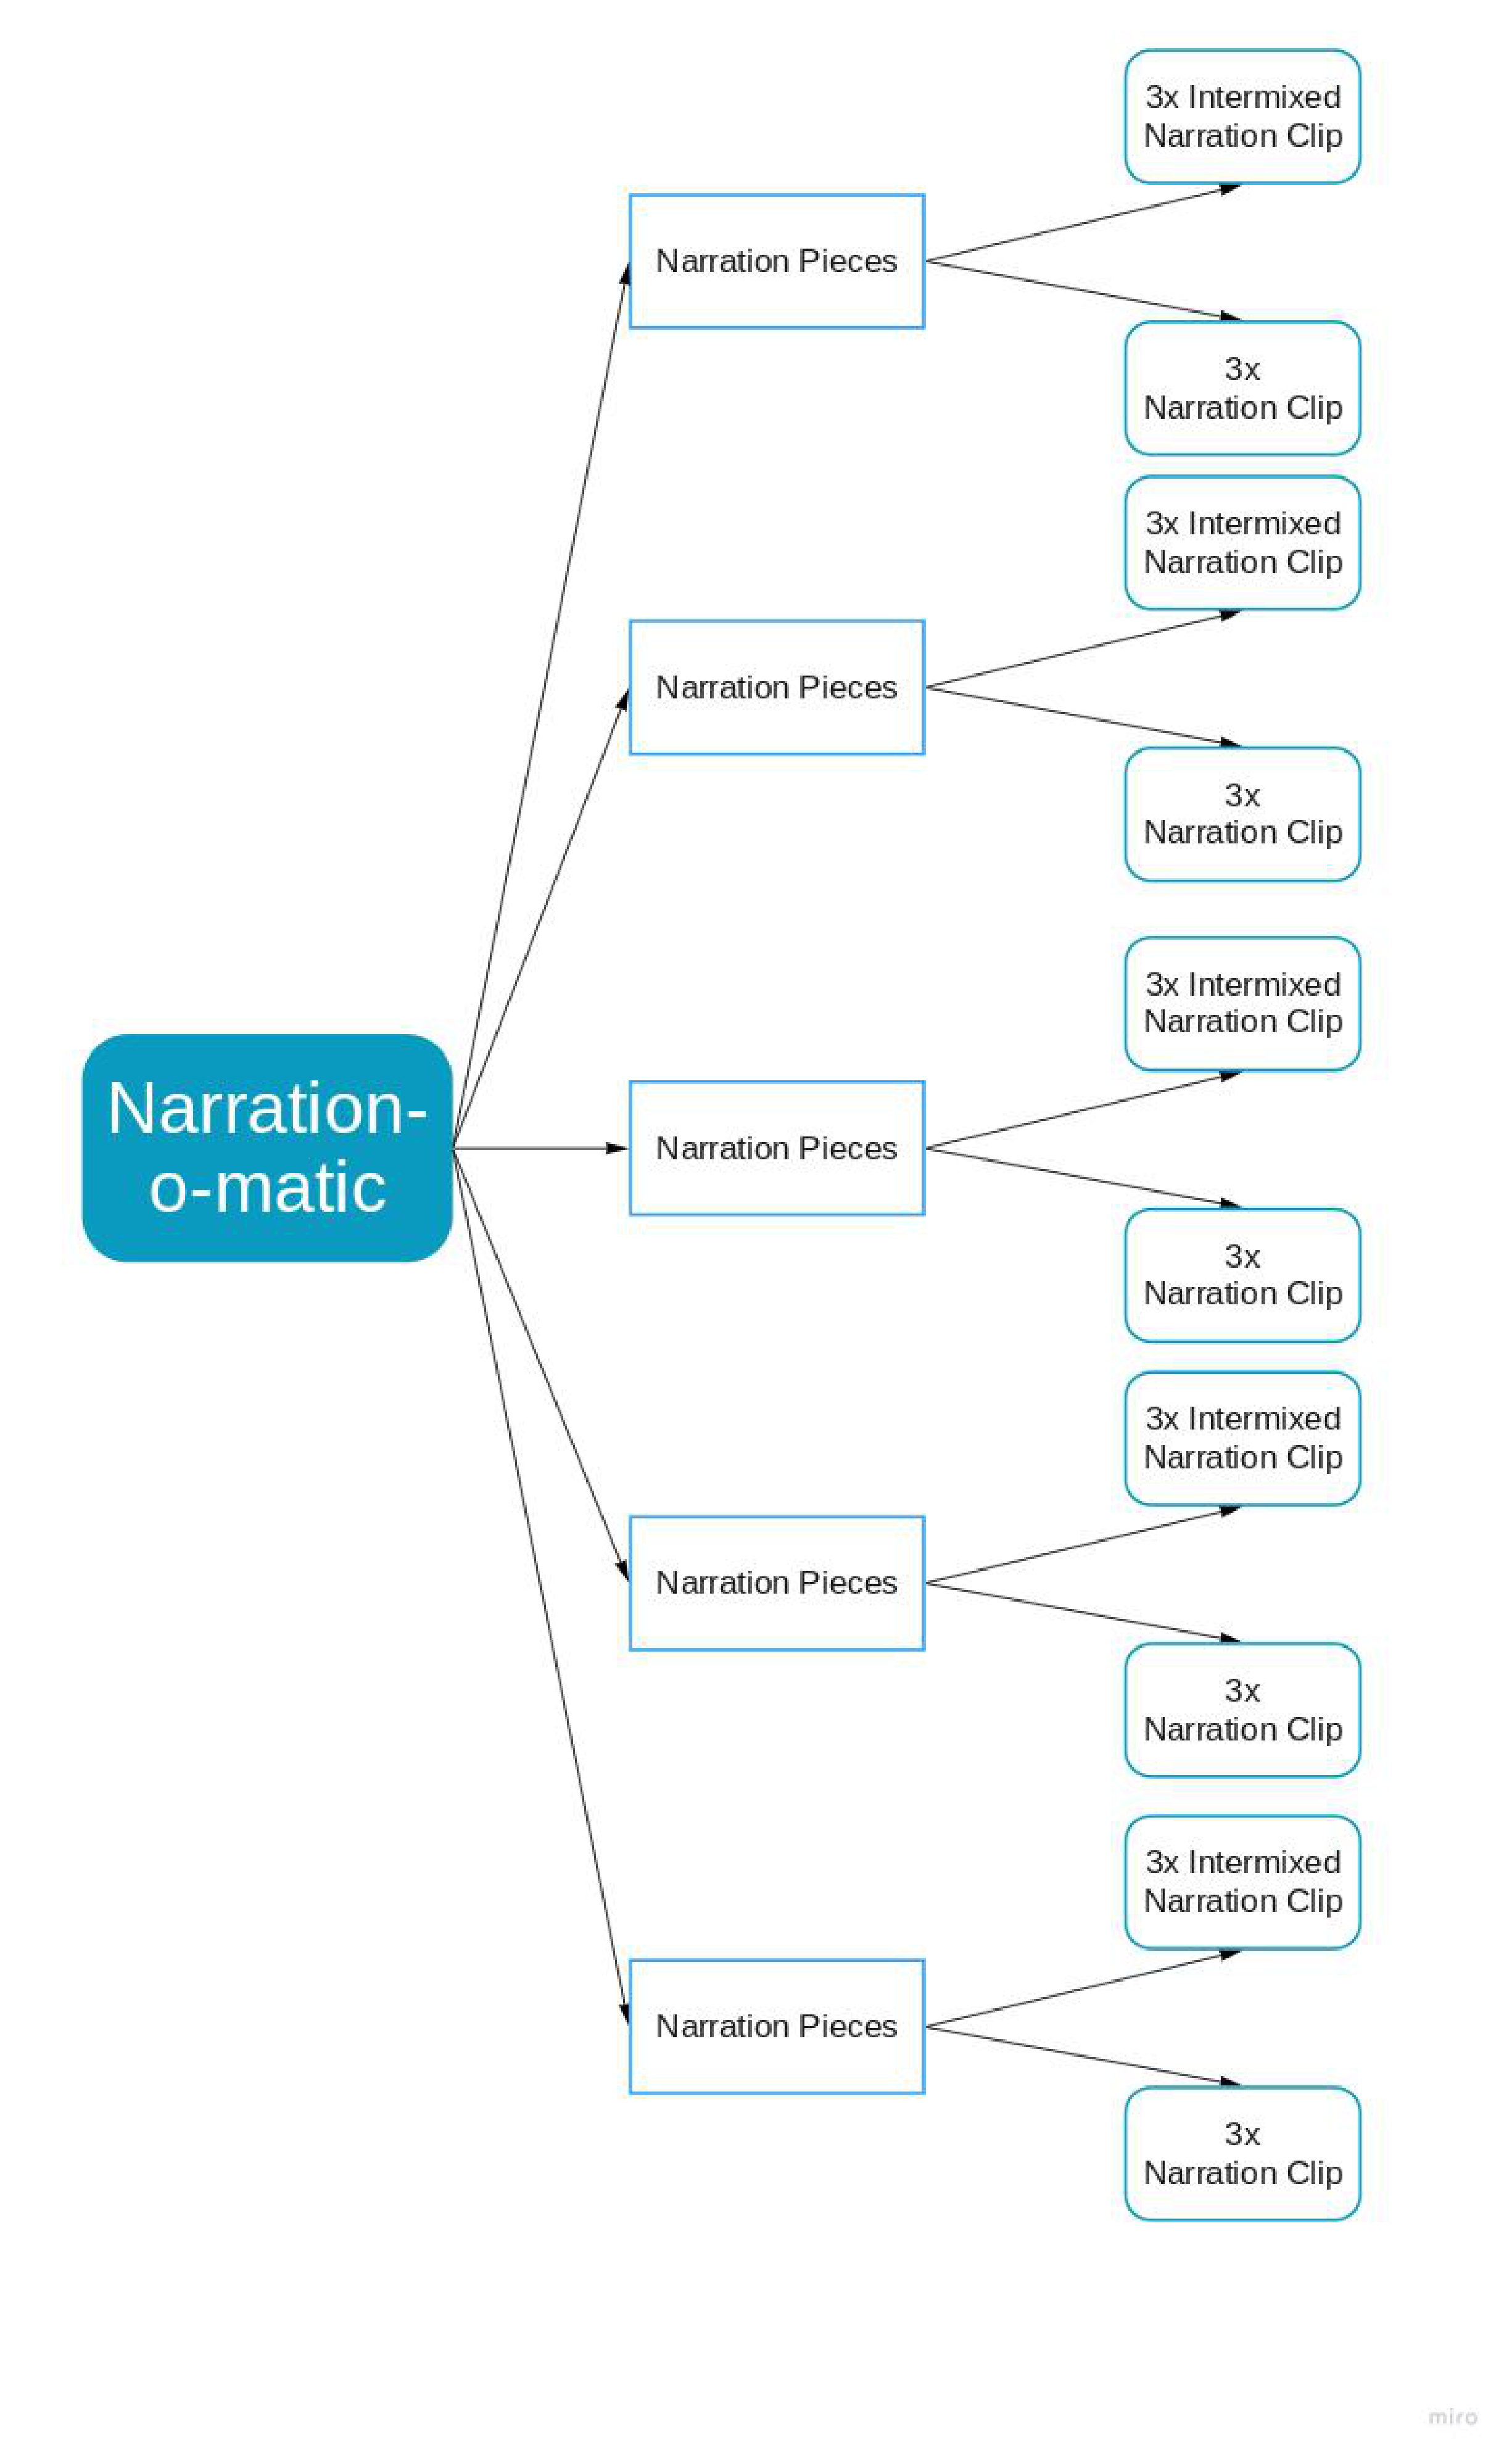
\includegraphics[width=0.9\linewidth]{figure/Implementation/Narration-o-matic-flowchart}
        \caption{The structure of the narration system called the narration-o-matic, showing the different narration pieces, each containing the intermixed (IM), and overloaded (OL) clips. With the addition of the introductory clip in the first piece.}
        \label{fig:narration-o-matic}
    \end{figure}
    
    \subsection{Narration}
        \todo{Maybe a section on the narration?}

\section{The Road}
    The roads (seen in \autoref{fig:screenshot_road}), modelled in blender (explained in \autoref{section:models}), are being placed in real time during the run of the program, continually being moved and replaced by new pieces, essentially making a never ending road. Hence making simpler to build the environment around the narration, instead of focusing on building road pieces.
    \begin{figure}[H]
        \centering
        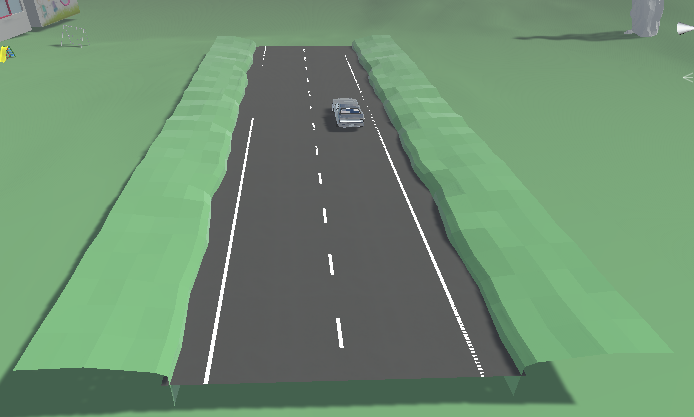
\includegraphics[width=0.8\linewidth]{figure/Implementation/screenshots/road.png}
        \caption{The roads used in the prototype, modelled using blender.}
        \label{fig:screenshot_road}
    \end{figure}
    
\section{The Environment}
Following the setup in \todo{design section talking about visual setup}, the visual zones were laid out in Unity, using the terrain editor. Using the built in solution from Unity, enabled for quick prototyping of visuals, and then moving the different elements for both the intermixed and overloaded version into two separate transforms, further sped up prototyping of visual elements.

A visual comparison can be seen in the mock ups in \autoref{fig:viz_IM}, and \autoref{fig:viz_OL}, giving an overview of the implemented visuals, and the differences between the intermixed, and overloaded version. There are the more subtle differences, like the \textit{JUSK} billboard being replaced by a more meat related one in the overloaded version, or the kindergarten replacing a statue. But there are also the more noticeable changes, like pigs and sheep completely missing from the intermixed version, or the houses not being in the overloaded version, this is all to balance out the content between the their desired ratios (as mention in \todo{design section talking about visual setup}).

\begin{multicols}{2}
    \begin{figure}[H]
        \centering
        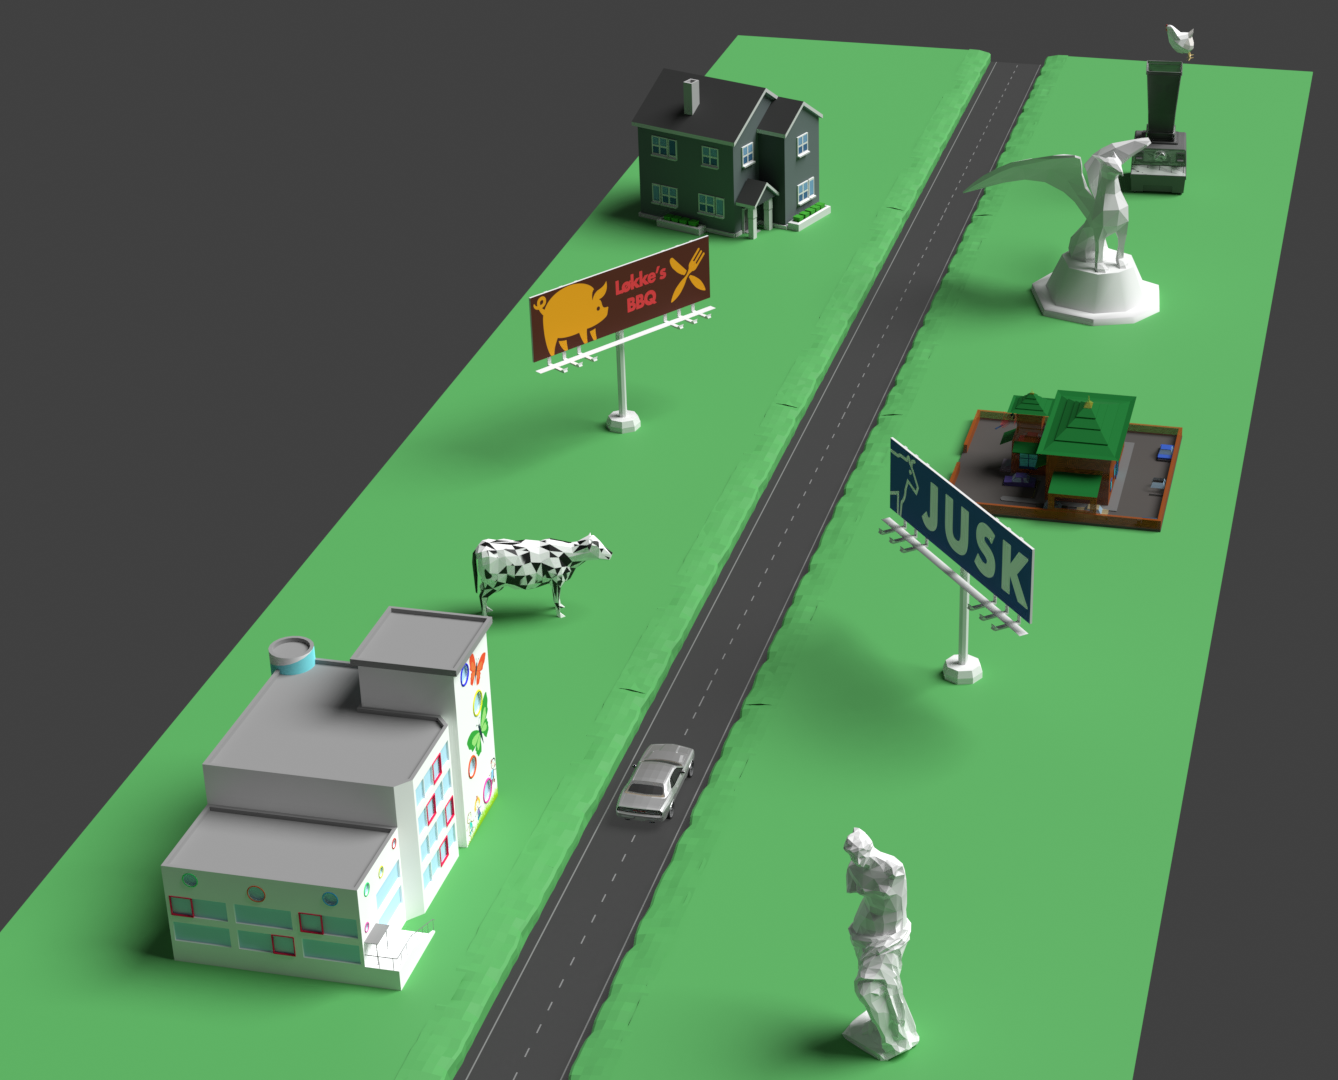
\includegraphics[width=0.95\linewidth]{figure/Implementation/Intermixed.png}
        \caption{A visualisation of the intermixed environment, with the populated zones.}
        \label{fig:viz_IM}
    \end{figure}
\columnbreak
    \begin{figure}[H]
        \centering
        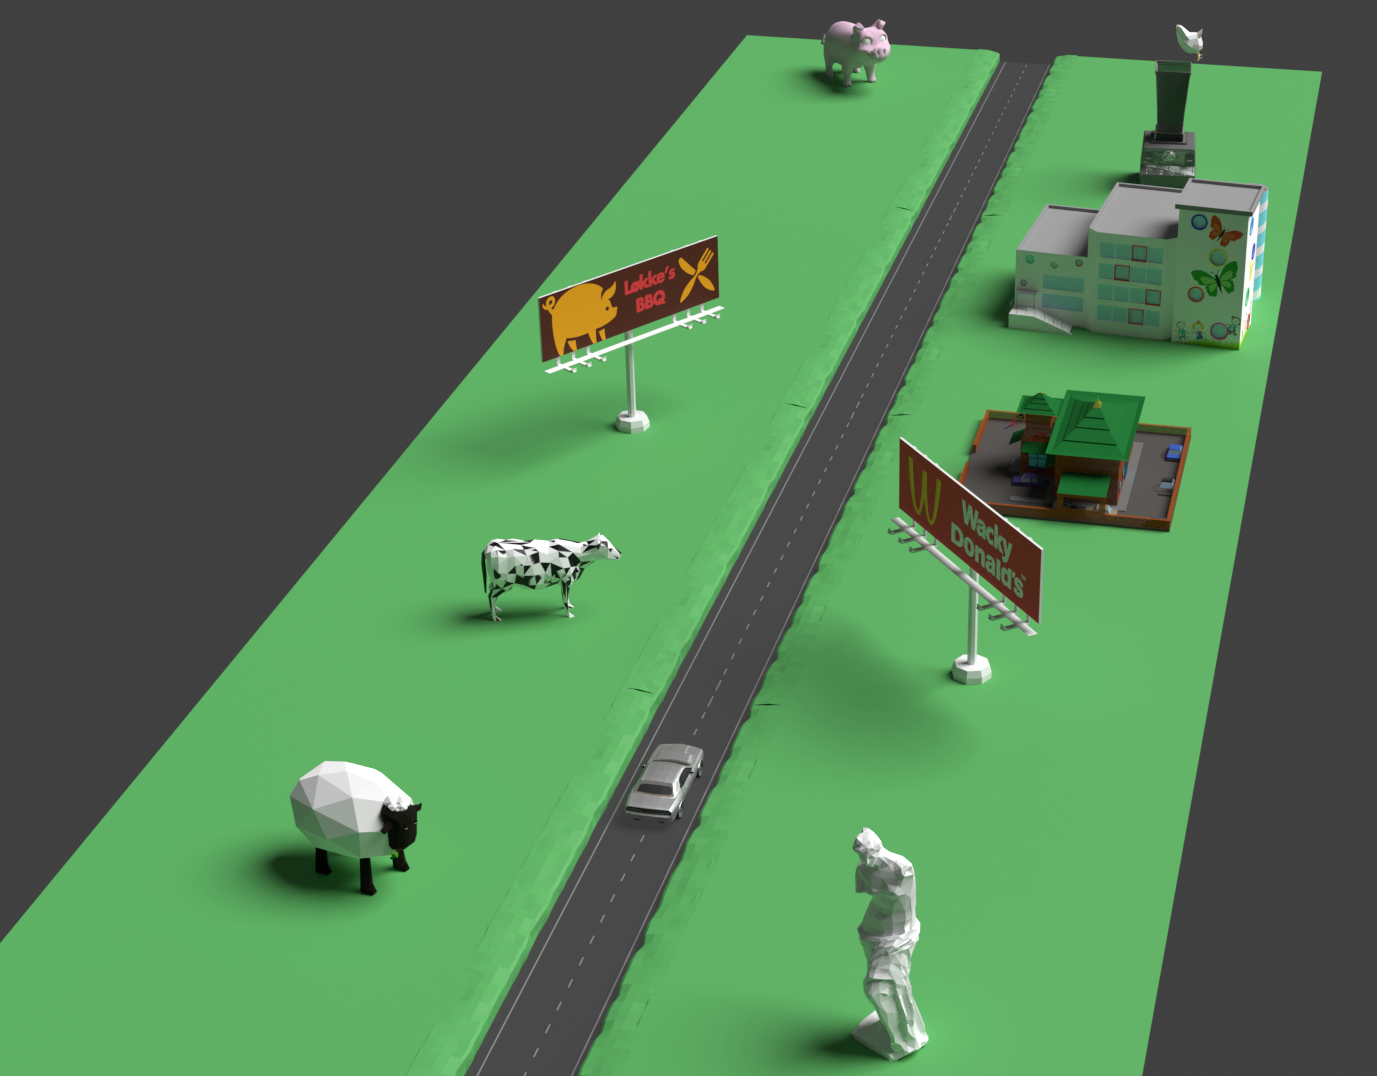
\includegraphics[width=0.98\linewidth]{figure/Implementation/Overloaded.png}
        \caption{A visualisation of the overloaded environment, with the populated zones.}
        \label{fig:viz_OL}
    \end{figure}
\end{multicols}

\section{Models}\label{section:models}
    The car model, and the rest of the used models in this prototype are royalty free, free assets downloaded from various sites, like turbosquid, and cgtrader. The car model needed to be cleaned, to make it an autonomous car. First, the steering wheel needed to be removed, then the pedals and the gear stick, and finally the dash had to be remade from scratch, to allow for the new additions to the interior, as seen in \autoref{fig:car_before}. These additions, as seen in \autoref{fig:car_after}, include the screen and burger flap, from which the burgers should magically come out.

\begin{multicols}{2}
    \begin{figure}[H]
        \centering
        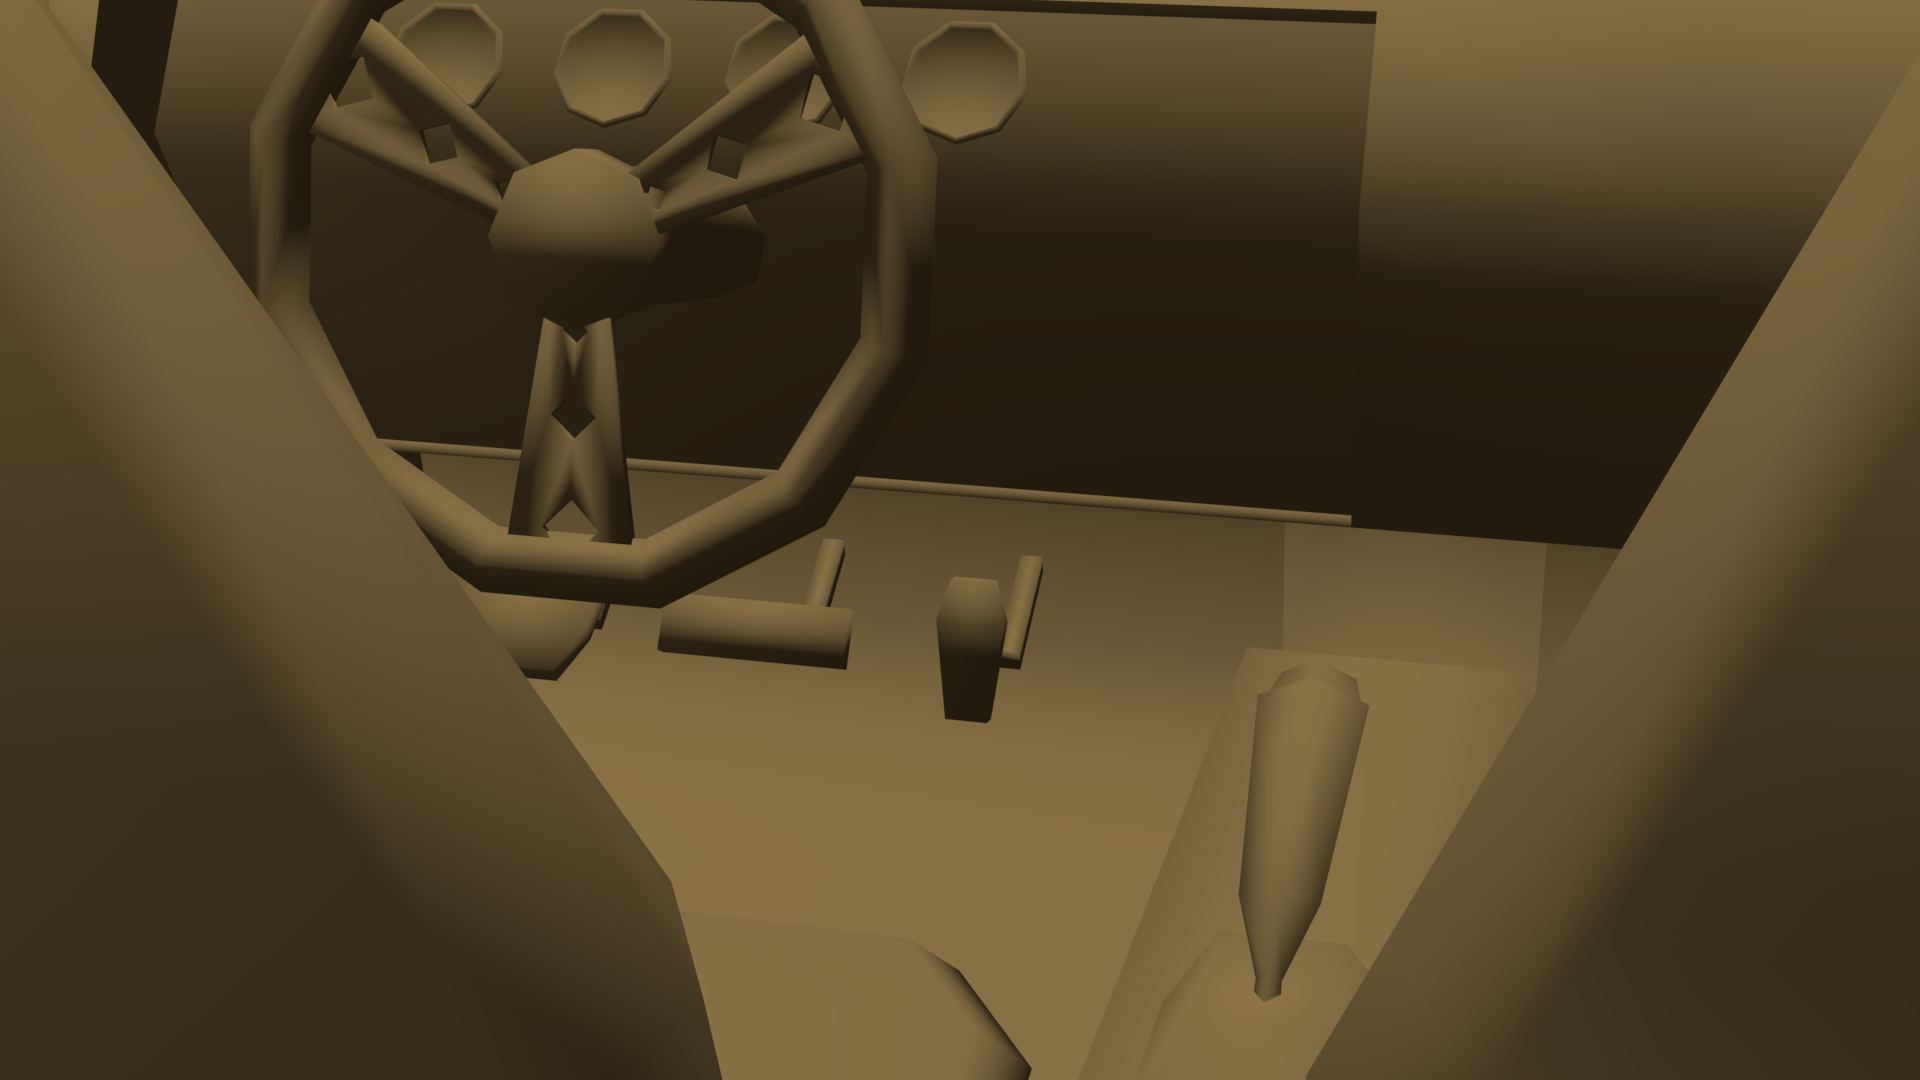
\includegraphics[width=0.99\linewidth]{figure/Implementation/car_before.png}
        \caption{Inside view of the car before the remodel, changing most of the interior to a simplified version.}
        \label{fig:car_before}
    \end{figure}
\columnbreak
    \begin{figure}[H]
        \centering
        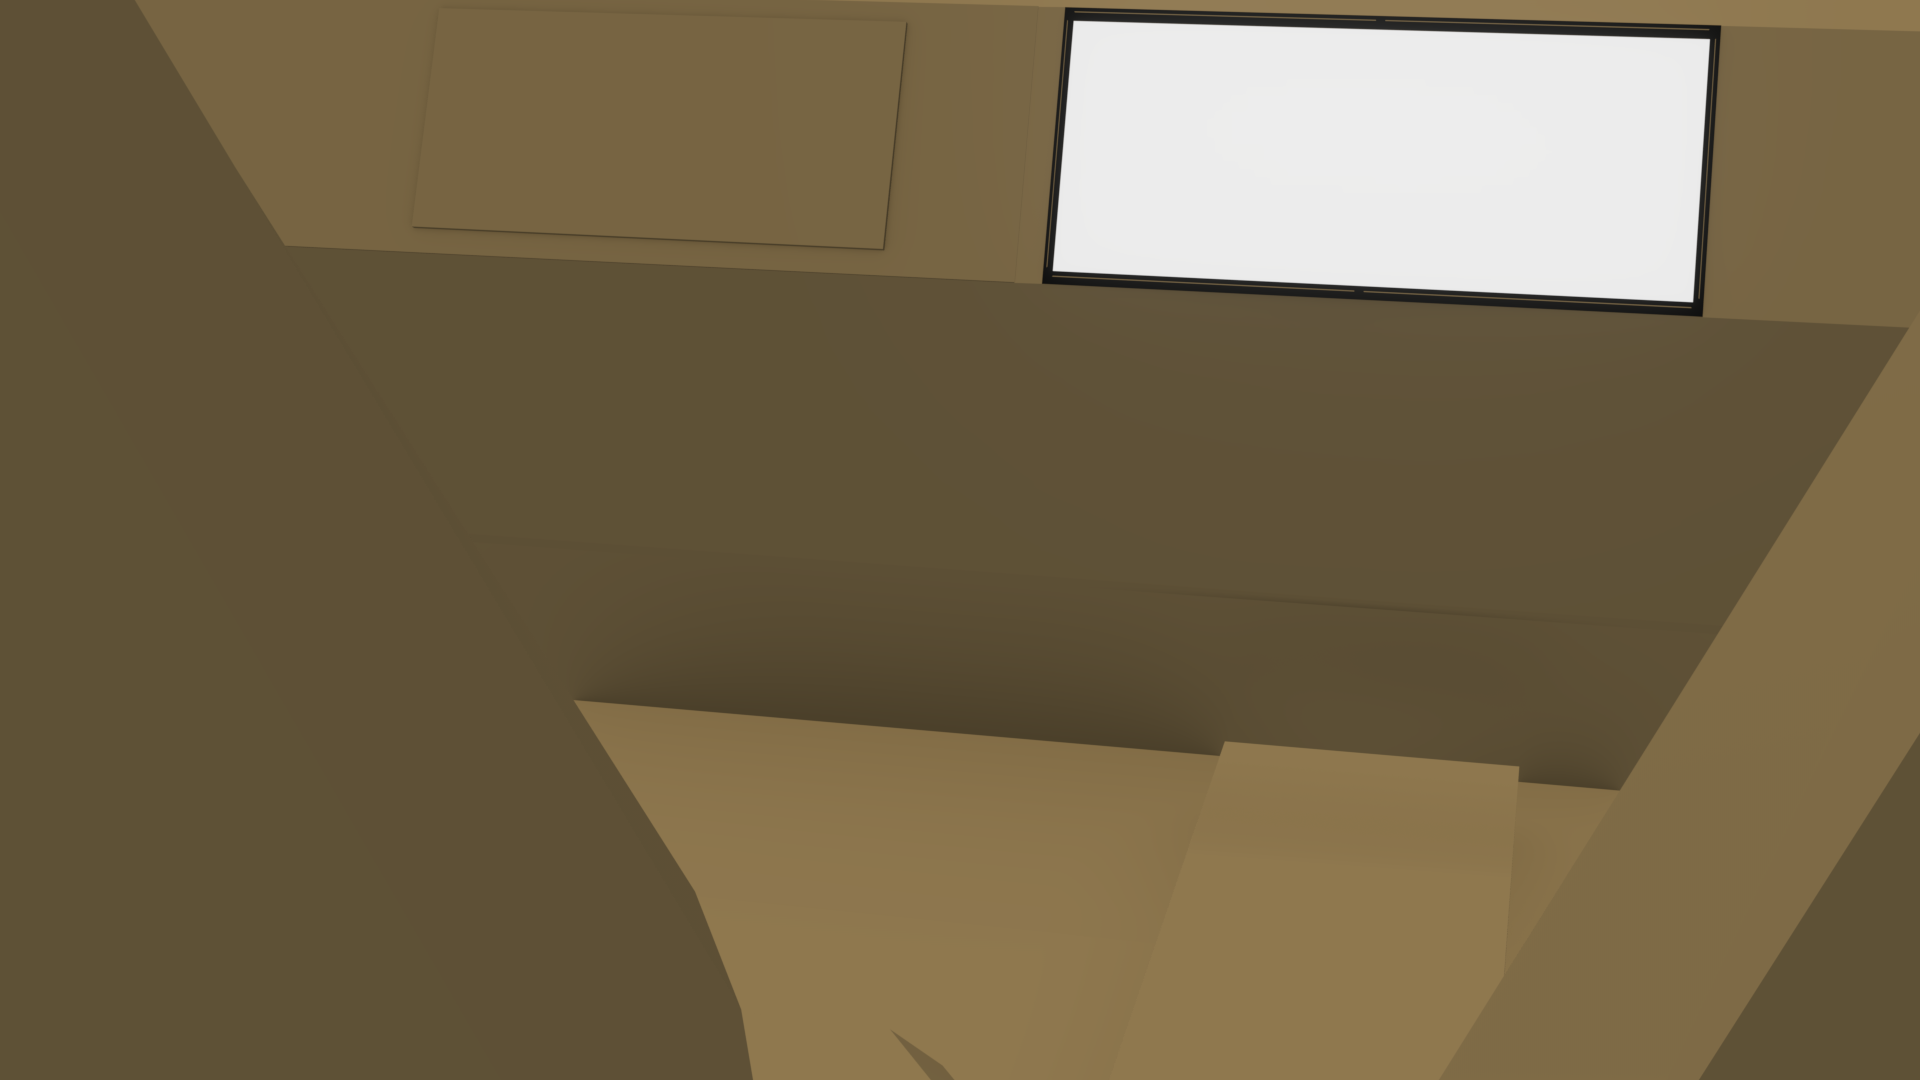
\includegraphics[width=0.99\linewidth]{figure/Implementation/car_after.png}
        \caption{Inside view of the car after the remodel, adding the screen and burger flap, while removing the elements that made the car not autonomous.}
        \label{fig:car_after}
    \end{figure}
\end{multicols}